\begin{section}{Molecular Simulation: History and Importance}

What are the functions of proteins in the body? How can we identify new and better drugs for improved
disease treatment, or optimal materials for designing efficient solar cells?
What are the microscopic mechanisms by which chemicals interact, undergo phase
transitions, or react to form entirely new species? Increasingly, these and other 
essential chemical questions can be addressed with the aid of computer
simulation, 
\cite{VanGunsteren1990,Hospital2015,Chen2015,Karplus2002,Ciccotti2014}
enabling us to, for example, peer into the detailed mechanisms of enzyme catalysis,
\cite{Warshel2003}
watch proteins fold,
\cite{Levitt1975,Lane2013,Piana2014,Perez2016}
virtually screen for novel drug candidates, 
\cite{DeVivo2016}
improve industrial materials,
\cite{Jiang2011,Maurin2016,Bereau2016}
and directly simulate hard-to-understand phase transformations at an atomistic level.
\cite{Kalikmanov2013,Wilding2001}
The question, of course, is: how?


To understand the link between computer simulation and obervable experimental properties
of interest,\footnotemark{} we first summarize several fundamental
physical principles
that help define the
scope and importance of molecular simulation.
One insight comes from the field of
statistical mechanics, where by the early 20\super{th} century it was discovered
that experimental observables, which we denote \obs, depend entirely on
a system's temperature, $T$, and the energies available to that system,
%
\begin{align}
\label{eq:intro-boltzmann}
\braket{\obs} = \frac{\sum\limits_n \obs_n \exp (-E_n/k_BT)}
                    {\sum\limits_n \exp (-E_n/k_BT)}.
\end{align}
%
Here the angle brackets denote that we're interested in some \emph{average}
value of the observable, the subscript $n$ indicates a possible state of the
system (defined in terms of the positions and momenta of all of the particles
in the system) with energy $E_n$ and value of the observable
$\obs_n$, 
and $k_B$ is Boltzmann's constant.\cite{allen1989computer}
 Technically,
this expression only holds for discrete systems at constant temperature,
however conceptually-similar expressions can be derived outside of these
assumptions. 
%TODO: Cite useful things here
Regadless, \cref{eq:intro-boltzmann} and related formulae show how, 
given knowledge of all possible energy states of a system, we can
have exact information for that system about any macroscropic properties of
interest. 

\footnotetext{
We've been intentionally vague about what these `experimental
properties of interest' might be, as the experimental properties one finds
important vary considerably between applications. 
To offer some concrete examples, drug discovery
studies are often interested in the binding free
energies between proteins and prospective drug
molecules,\cite{DeVivo2016,Bereau2016}
and the optimization of putative solar cell materials often focuses on
open circuit voltages and/or short-circuit currents.\cite{Bereau2016}
}

In practice, most chemical systems contain large numbers of particles, and
the number of avaiable system states become intractably large. Thus in all but the
simplest cases, 
\cref{eq:intro-boltzmann} is overly difficult to solve by mere enumeration and
averaging of states.\cite{allen1989computer}
Fortunately,
several crucial scientific advances 
%% (one at the turn of the 20\super{th}
%% century,\cite{boltzmann1898vorlesungen} and others in the 1950s and 60s\cite{allen1989computer})
paved the way to reformulate the relationship between $\braket{\obs}$ and $E_n$ in terms
of known --- and tractable --- problems in such disparate fields as classical dynamics
and probability theory.
The connection to classical dynamics began at the turn of the 20\super{th} century,
when Ludwig Boltzmann proposed his now-famous `ergodic' hypothesis.\cite{boltzmann1898vorlesungen} Over sufficiently
long time periods, according to Boltzmann, the `ensemble average' defined in \cref{eq:intro-boltzmann} becomes
identical to the `time-average' that results from studying the system's
dynamical behavior:
%
\newcommand{\tobs}{\ensuremath{t_{\text{obs}}}\xspace}
\begin{align}
\label{eq:intro-md}
\braket{\obs} = \braket{\obs}_{\text{time}} 
= \braket{\obs(\bm{\Gamma}(t)}_{\text{time}} 
= \lim_{t_{\text{obs}} \to \infty} \frac{1}{t_{\text{obs}}}
\int\limits_0^{t_{\text{obs}}}
\obs(\bm{\Gamma}(t)) dt .
\end{align}
%
Here we have used $\bm{\Gamma}(t)$ to denote the collective positions and
momenta that define the state of the system as a function of time, and \tobs
to indicate the length of time over which we average the system's
properties.\cite{allen1989computer} The
right-hand side of \cref{eq:intro-md} proves remarkably useful: so long as we know and can
solve for the equations of motion that govern a given system's behavior, we can
simulate the time evolution of that system until the r.h.s. of
\cref{eq:intro-md} converges, and in doing so obtain an average value for any desired
property of that system. 

Boltzmann's ergodic hypothesis wasn't fully taken advantage of until the 1960s
and 70s, as the laws of motion governing quantum mechanical systems can often
be incredibly complex. \emph{Classical} mechanics, on the other hand, is
governed simply by Newton's laws of motion,
%
\begin{align}
\label{eq:intro-newton}
- \frac{d E(\bm x)}{d \bm x} \equiv \bm F(\bm x) = m \ddot{\bm x}, 
\end{align}
%
with $\bm x$ as a position vector, $m$ a mass, and $F$ the force acting on a
particle. Thus for classical particles, we need only know the forces operating
on each particle (which is a direct function of the system's energy) to solve for the
time-dependent positions, momenta, and (ultimately) properties of a system.
Critically, even though atomic behavior is strictly quantum mechanical, it was
discovered that a classical mechanical description of the atomic motions could
often yield satisfactory information, particularly for heavier atoms at higher
temperatures.
\cite{Karplus2014}
As a result of this highly important insight (indeed, Karplus, Levitt, and
Warshel won the Nobel prize for these ideas and related
work),\cite{Karplus2014} it soon became possible to study both kinetic and
thermodynamic properties of a wide range of molecular systems, historically beginning with monatomic
liquids in 1964, and soon leading to the first polymer and protein simulations in 1975 and
1977, respectively.\cite{VanGunsteren1990} Ever since these first studies, the field of \md has 
increasingly become a preeminent tool in the investigation and prediction of chemical
phenomena.

Around the same time as \md was being developed and popularized as a `dynamics' solution to
\cref{eq:intro-boltzmann}, a separate group of
researchers\cite{Metropolis1953} found a way to
formulate \cref{eq:intro-boltzmann} as a sampling problem based in probability
theory: 
\cite{Harrison2010,allen1989computer}
%
\begin{align}
\label{eq:intro-mc}
\braket{\obs} = \braket{\obs}_{\text{ens}} 
= \lim_{\tau_{\text{obs}} \to \infty} \frac{1}{\tau_{\text{obs}}}
\sum\limits_{\tau = 1}^{\tau_{\text{obs}}}
\obs(\bm{\Gamma}(\tau))
\end{align}
%
In contrast to \cref{eq:intro-boltzmann}, \cref{eq:intro-mc} is the average
over a total number of observations, ${\tau_{\text{obs}}}$, taken of the
system and its properties randomly sampled, according to some probability
distribution $\rho$, over all states of the system.  The key technique that
defines MC is known as `importance sampling': provided we cleverly choose our
probability distribution, $\rho$, to be identical to the Boltzmann
distribution, $\rho \propto \exp (-E_n/k_BT)$, the right-hand side of
\cref{eq:intro-mc} converges fairly rapidly as a function of
${\tau_{\text{obs}}}$.  The interested reader is directed to
\citet{allen1989computer} for detailed information
on the exact techniques, algorithms, and practical concerns involved in
importance sampling.  
%
Regardless of which specific technique is used, however, both
\md and \mc methods
enable us to calculate thermodynamic (and sometimes kinetic) properties of
interest based solely on knowledge of the energy of a system as a function of
the system state, enabling molecular simulation as we know it today.
%}




%% ========================================================
%% 
%% 
%% 
%% The aim of computer simulations of molecular systems is to compute macroscopic
%% behavior from microscopic interactions.
%% The main contributions a microscopic consideration can offer are (1) the
%% understanding and (2) interpretation of experimental results, (3)
%% semiquantitative estimates of experimental re- sults, and (4) the capability
%% to interpolate or extrapolate experimental data into regions that are only
%% difficultly accessible in the laboratory.
%% \cite{VanGunsteren1990}
%% 
%% The design of materials guided by computation is expected to
%% lead to the discovery of new materials, reduction of materials development
%% time and cost, and the rapid evolution of new materials into products.1
%% \cite{Chen2015}
%% 
%% Simulations can provide the ultimate detail concerning individ- ual particle
%% motions as a function of time. Thus, they can be used to address specific
%% questions about the properties of a model sys- tem, often more easily than
%% experiments on the actual system. For many aspects of biomolecular function,
%% it is these details that are of interest (for example, by what pathways does
%% oxygen enter into and exit from the heme pocket in myoglobin?). Of course,
%% experiments play an essential role in validating the simulation methodology:
%% comparisons of simulation and experimental data serve to test the accuracy of
%% the calculated results and to provide criteria for improving the methodology.
%% This is particularly important because theoretical estimates of systematic
%% errors inherent in simulations have not been possible — that is, the errors
%% introduced by the use of empirical potentials are difficult to quantify
%% ...
%% There are three types of applications of simulation methods in the
%% macromolecular area, as well as in other areas involving mesoscopic systems.
%% The first uses simulation simply as a means of sampling configuration space.
%% This is involved in the utiliza- tion of molecular dynamics, often with
%% simulated annealing pro- tocols, to determine or refine structures with data
%% obtained from
%% experiments, as mentioned above. The second uses simulations to obtain a
%% description of the system at equilibrium, including structural and motional
%% properties (for example, atomic mean- square fluctuation amplitudes) and the
%% values of thermodynamic parameters. For such applications, it is necessary
%% that the simula- tions adequately sample configuration space, as in the first
%% appli- cation, with the additional condition that each point be weighted by
%% the appropriate Boltzmann factor. The third area uses simula- tions to examine
%% the actual dynamics. Here not only is adequate sampling of configuration space
%% with appropriate Boltzmann weighting required, but it must be done so as to
%% correctly repre- sent the development of the system over time. For the first
%% two areas, Monte Carlo simulations can be used, as well as molecular dynamics.
%% By contrast, in the third area where the motions and their development with
%% time are of primary interest, only molec- ular dynamics can provide the
%% necessary information. The three sets of applications make increasing demands
%% on simulation methods as to their required accuracy and precision.
%% \cite{Karplus2002}

\end{section}
\begin{section}{Molecular Simulation: Challenges and Unanswered Questions}

Recent successes in \md and \mc simulations
have shown great promise for using molecular simulation in the understanding,
interpretation, and even prediction of experimental
results,\cite{VanGunsteren1990}
making simulation a powerful complement to traditional experimental tools.
\cite{Hospital2015,Karplus2002,Bereau2016,Chen2015,Maurin2016,Jiang2011,Schneider2005,Jorgensen2004}
Nevertheless, accurate and insightful molecular simulation
depends on success in the following three critical aspects of any \md/\mc simulation:
\cite{Lane2013}
%
\begin{enumerate}
\item We must be able to accurately and efficiently quantify the potential
energy, $E_n$, of any state $n$ of the system that might get sampled by the
\md/\mc simulation. 
\cite{Ballone2014,Lopes2015,Saunders2013,DeCarvalho2014}
Henceforth we will collectively refer to these energies, given as a function
of the system state $\bm \Gamma$, as the \pes of a system (Some visual
examples of representative \glspl{pes} are shown in \cref{fig:intro-pes}).
\item We must be able to obtain a representative sample of all states of the system over a sufficiently long timescale
(commensurate with the timescale(s) of the chemical phenomena of interest) so as
to obtain converged property predictions.
\cite{Lei2007,Grossfield2010,Theodorou2010}
This class of problems is often referred to simply as `sampling issues'.
\item Especially when interested in \emph{interpreting} chemical phenomena, we must be
able to analyze the results of a simulation in such a way as to garner
detailed, chemically-intuitive insight into the problem at hand.
\cite{E2010,Pande2010,Rohrdanz2013}
While this task is relatively straightforward for homogeneous liquids and
other `simple' systems,
it can become decidedly
difficult for analyzing complex properties and mechanisms, such as with using
simulation to investigate protein folding mechanisms.
\end{enumerate}
Though our focus in this dissertation will be on the first point (that of
computing potential energies for molecular simulation), all three 
aspects of molecular simulation are challenging in their own right, and form
highly active and important areas of research. 
\cite{Ciccotti2014} 
Moreover, there is significant interplay between these areas in terms of
research development.
As an example, improvements in sampling methods often lead to increased computational
efficiency, thereby enabling use of more accurate (but more costly)
representations of the \pes. Conversely, the next section will discuss how the development of
cost-effective potential energy functions is often necessary for
running simulations over long enough time scales to ensure representative
sampling and robust interpretation of the simulation results. Clearly, insofar
as molecular simulation is concerned, both
accuracy and computational efficiency are of paramount importance. 

%%%%%%%%%%%%%%%%%%%%%%%%%%%%%%%%%%%%%%%%%%%%%%%%%%%%%
\begin{figure}
\centering
    \begin{subfigure}[t]{0.75\textwidth}
        \centering
        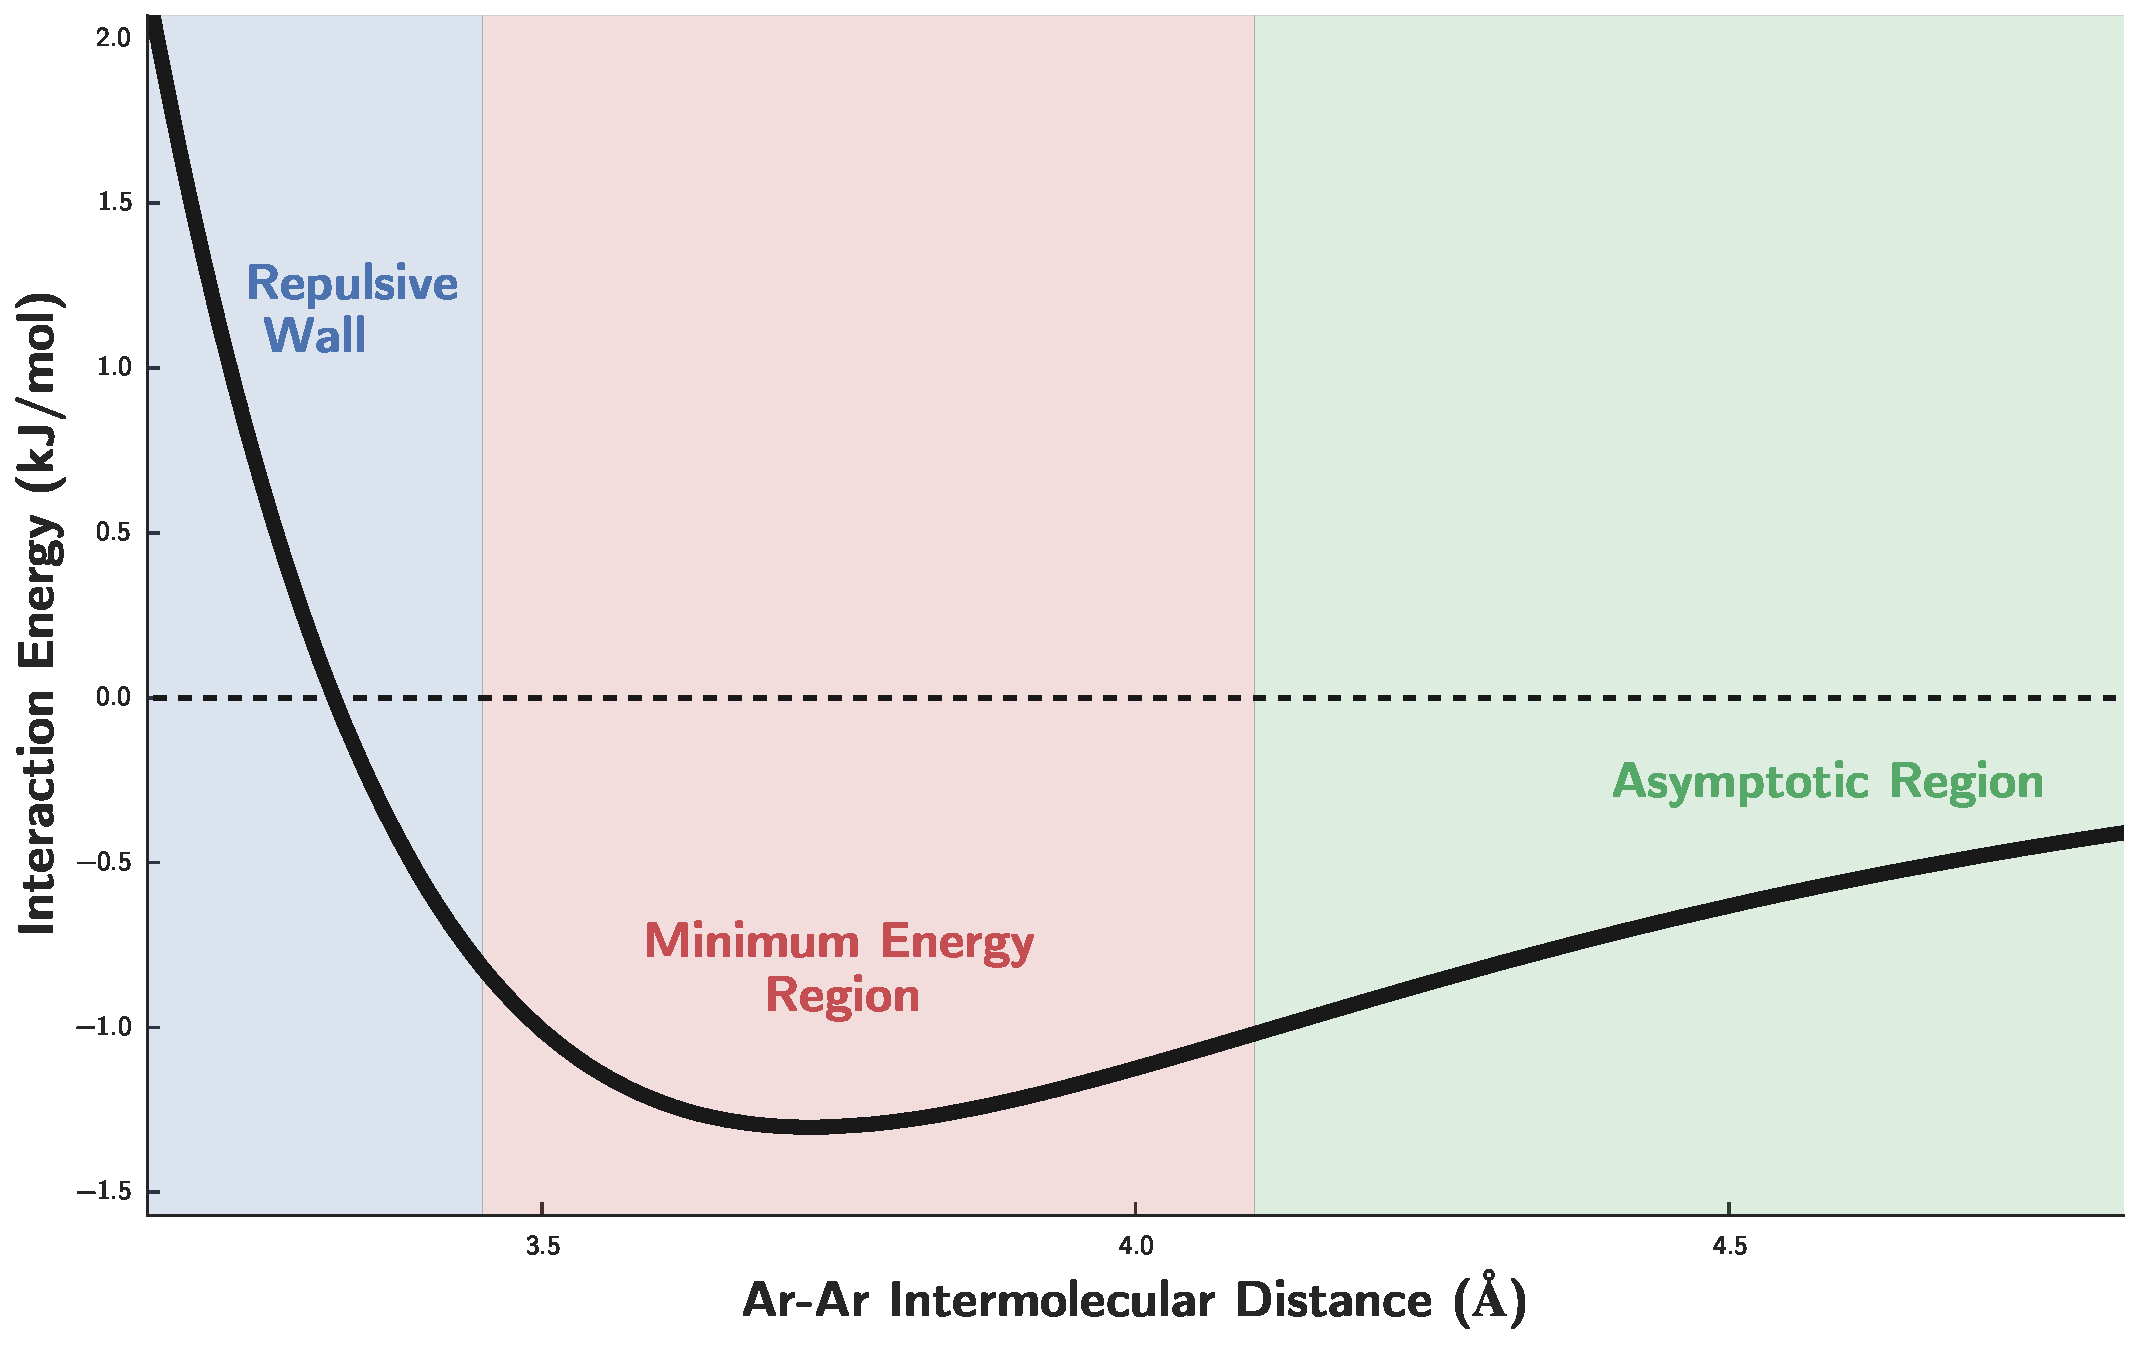
\includegraphics[width=1.0\textwidth]{workflow/generalized_pes.pdf}
        \caption{One-dimensional \pes for the argon dimer.}
    \end{subfigure}
    ~ 
    \begin{subfigure}[t]{0.75\textwidth}
        \centering
        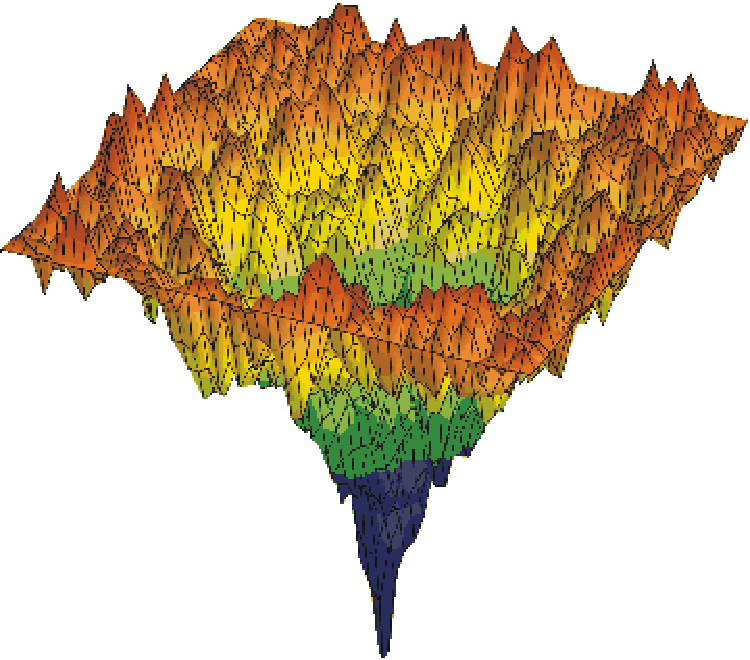
\includegraphics[width=1.0\textwidth]{intro/protein_pes.pdf}
        \caption{Three-dimensional representation of an $N$-dimensional \pes
            for a protein. Copied under a CC license from \citet{Chaplin2017} }
    \end{subfigure}%
\caption{Simple and complex \acrlongpl{pes} for molecular systems.}
\label{fig:intro-pes}
\end{figure}
%%%%%%%%%%%%%%%%%%%%%%%%%%%%%%%%%%%%%%%%%%%%%%%%%%%%%

In the pursuit of increasingly accurate, insightful, and predictive molecular
simulation, it is clear that we must be able to quantitatively represent the
\pes of any molecular system, and, furthermore, that our mathematical
representation of this \pes must be sufficiently accurate and cost-effective so
as to enable simulation that is chemically insightful (given the type of
simulation analysis required for a particular problem or application) and
computationally affordable (in accordance with the length of molecular simulation that will
need to be run in order to appropriately deal with any sampling issues). 
Bearing these stipulations in mind, we can now broadly state the guiding
question for this dissertation: in the pursuit of
accurate and insightful molecular simulation, how can we optimally
obtain a mathematical description of the \pes?

\end{section}
